
\documentclass[letterpaper,12pt]{article}
% \documentclass[a4paper,12pt]{article}
% twocolumn letterpaper 10pt 11pt twoside

% for other type sizes, 8, 9, 10, 11, 12, 14pt, 17pt, 20pt
% \documentclass[14pt]{extarticle}
% also extbook, extletter available
% \usepackage{extsizes}

%\usepackage{endnotes}
% then put \theendnotes where you want them

\usepackage{times}
\usepackage{xspace}
%\usepackage{alltt}
\usepackage{fancyvrb}  % \begin{Verbatim}[fontsize=\small]
% or [fontsize=\footnotesize]

%\usepackage{latexsym}  % \LaTeX{} for LaTeX;  \LaTeXe{} for LaTeX2e
%\usepackage{mflogo}    % \MF{}  for METAFONT;  \MP for METAPOST
\usepackage{url}       % \url{http://www.xrce.xerox.com/people/beesley}
%\usepackage{lscape}    % allows \begin{landscape} ... \end{landscape}

%\usepackage{tipa}
%\include{ipamacros}  % my macros to allow same input for DA and IPA
%\usepackage{desalph}
%\usepackage{arabtex} % see usepackage{buck} and setcode{buck} below
%\usepackage{buck}
%\usepackage{mxedruli}

%\usepackage{epsfig}
%\usepackage{pslatex}  % make whole doc. use postscript fonts

\usepackage{upquote}
% affects \verb and verbatim
% to get straight quotes, straight single quote, straight double
% quotes in verbatim environments

% parallel columns, see also multicol
%\usepackage{parcolumns}
%...
%\begin{parcolumns}[<options>]{3}
%\colchunk{ column 1 text }
%\colchunk{ column 2 text }
%\colchunk{ column 3 text }
%\colplacechunks
%...
%\end{parcolumns}


% for more of these names, see Guide to LaTeX, p. 351
%\providecommand*{\abstractname}{}     % in case the style defines one
%\renewcommand*{\abstractname}{Transcriber notes}
%\renewcommand*{\figurename}{Figure}
%\renewcommand*{\tablename}{Table}
%\renewcommand*{\bibname}{Bibliography}
%\renewcommand*{\refname}{References}

\providecommand{\acro}{}\renewcommand{\acro}{\textsc}
\providecommand{\defin}{}\renewcommand{\defin}{\textsc}

\newcommand{\key}{\textbf}
\newcommand{\translit}{\texttt}

% forced pagebreak
%\newpage

%\usepackage{ulem}
%    \uline{important}   underlined text
%    \uuline{urgent}     double-underlined text
%    \uwave{boat}        wavy underline
%    \sout{wrong}        line drawn through word (cross out, strike out)
%    \xout{removed}      marked over with //////.
%    {\em phasized\/}  | In LaTeX, by default, these are underlined; use
%    \emph{asized}     | \normalem or [normalem] to restore italics
%    \useunder{\uwave}{\bfseries}{\textbf}
%                        use wavy underline in place of bold face


%                        \usepackage{natbib}
%\usepackage[authoryear]{natbib}
% compatible with \bibliographystyle{plain}, harvard, apalike, chicago, astron, authordate

%\citet for "textual"   \citet{jon90} ->  Jones et al. (1990)
%\citet[before][after]{key} e.g. \citet[see][p.~47]{jon90} --> 
%         see Jones et al.(1990, chap. 2)
%\citet[chap. 2]{jon90}	    -->    	Jones et al. (1990, chap. 2)
%\citet[after]{key}

%   citep for "parenthetical"
%\citep{jon90}	    -->    	(Jones et al., 1990)
%\citep[chap. 2]{jon90}	    -->    	(Jones et al., 1990, chap. 2)
%\citep[see][]{jon90}	    -->    	(see Jones et al., 1990)
%\citep[see][chap. 2]{jon90}	    -->    	(see Jones et al., 1990, chap. 2)

%\citep for "parenthetical" (author's name in parens)
%\citep  similar
%
%\citet*{key}  list all authors, not just et.al
%\citetext{priv.\ comm.} comes out as (priv. comm.)
%
%just the author or year
%\citeauthor{key} comes out as "Jones et al."
%\citeauthor*{key} comes out as "Jones, Sacco and Vanzetti"
%\citeyear{key}   comes out as 1990
%\citeyearpar{key}            (1990)
%
%Rare stuff:
%use \Citet and \Citep for exceptional forcing of initcap on names
%like 'della Robbia' when it appears first in a sentence.
%
%\citealt like \citet but without parens
%\citealp like \citep but without parens
%


% fancyheadings from The Book (old, obsolete, I think)
%\usepackage{fancyheadings}
%\pagestyle{fancyplain}
% remember the chapter title
%\renewcommand{\chaptermark}[1]{\markboth{#1}{}}
%\renewcommand{\sectionmark}[1]{\markright{\thesection\ #1}}
%\lhead[\fancyplain{}{\small\scshape\thepage}]{\fancyplain{}{\small\scshape\rightmark}}
%\rhead[\fancyplain{}{\small\scshape\leftmark}]{\fancyplain{}{\small\scshape\thepage}}
%\cfoot{}

% new fancyhdr package
%\usepackage{fancyhdr}
%\pagestyle{fancy}
%\fancyhead{}

%% L/C/R denote left/center/right header (or footer) elements
%% E/O denote even/odd pages

%% \leftmark, \rightmark are chapter/section headings generated by the 
%% book document class

%\fancyhead[LE,RO]{\slshape\thepage}
%\fancyhead[RE]{\slshape \leftmark}
%\fancyhead[LO]{\slshape \rightmark}
%\fancyfoot[LO,LE]{\slshape Short Course on Asymptotics}
%\fancyfoot[C]{}
%\fancyfoot[RO,RE]{\slshape 7/15/2002}

% another example
%\fancyhead[LE]{\thepage}
%\fancyhead[CE]{\bfseries Beesley}
%\fancyfoot[CE]{First Draft}
%\fancyhead[CO]{\bfseries My Article Title}
%\fancyhead[RO]{\thepage}
%\fancyfoot[CO]{For Review and Editing Only}
%\renewcommand{\footrulewidth}{0.4pt}

% \vspace{.5cm}
% c, l, r, p{1cm}
%\begin{tabular}{}
%\hline
%   &  &  &   \\
%\hline
%\end{tabular}
% \vspace{.5cm}


% bigbox -- puts a box around a float
% for {figure}, {table} or {center}

\newdimen\boxfigwidth  % width of figure box

\def\bigbox{\begingroup
  % Figure out how wide to set the box in
  \boxfigwidth=\hsize
  \advance\boxfigwidth by -2\fboxrule
  \advance\boxfigwidth by -2\fboxsep
  \setbox4=\vbox\bgroup\hsize\boxfigwidth
  % Make an invisible hrule so that
  % the box is exactly this wide
  \hrule height0pt width\boxfigwidth\smallskip%
% Some environments like TABBING and other LIST environments
% use this measure of line size -
% \LINEWIDTH=\HSIZE-\LEFTMARGIN-\RIGHTMARGIN?
  \linewidth=\boxfigwidth
}
\def\endbigbox{\smallskip\egroup\fbox{\box4}\endgroup}


% example
% \begin{figure}
%   \begin{bigbox}
%     \begin{whatever}...\end{whatever}
%     \caption{}
%     \label{}
%   \end{bigbox}
% \end{figure}
% 
% N.B. put the caption and label inside the bigbox

\usepackage{graphicx}
% Sample Graphics inclusion; needs graphicx package
%\begin{figure}[ht]
%\begin{bigbox}
%\centering
%\includegraphics{foobar.pdf}   # e.g. PNG, PDF or JPG, _not_ EPS
%\caption{}
%\label{lab:XXX}
%\end{bigbox}
%\end{figure}

%\pagestyle{empty}  % to suppress page numbering

% turn text upside down
%\reflectbox{\textipa{\textlhookp}}
% prevent line break:   \mbox{...}

\hyphenation{hy-po-cri-tical ri-bald}

%%%%%%%%%%%%%%%%%%%%  title %%%%%%%%%%%%%%%%%%%%%%%%%%%%%%

\title{Runtime Code for Finite-state Networks Produced by Kleene}
\author{Kenneth R.~Beesley\\Second Draft}

% to override automatic "today" date
\date{7 January 2011}

%\usepackage{makeidx}
%\makeindex
% see \printindex below in the document
%\usepackage{showidx}   % print proofs showing indexed locations!!!

%%%%%%%%%%%%%%%%%%%%%% document %%%%%%%%%%%%%%%%%%%%%%%%%%

\begin{document}
\maketitle

%\tableofcontents
%\listoffigures
%\listoftables

\begin{abstract}
This document, which will no doubt evolve, explains basic terminology and issues required
to understand the differences between the Kleene \emph{development code}, and the separate C++
\emph{runtime code} that will be required to 1) read in the finite-state networks (also known in
OpenFst terminology as FSTs) created
using Kleene, and 2) apply those networks to real data.

This document was largely written in May of 2009 and does not include any
mention of later developments, including Phil Sours' runtime code for
recursive transition networks (\acro{rtn}s).
\end{abstract}

\newpage

\section{Introducing Runtime Code}

\subsection{What is Runtime Code?}

I have \emph{never} been able to explain Runtime Code very well to most
of my colleagues, 
whether at Inxight, Business Objects or \acro{sap}.  This
is both disappointing and dangerous, because so much depends on it.  However, there is nothing new about runtime
code in our tradition.  Very sophisticated runtime code was written at Inxight, by Inxight employees, e.g.\@ to
apply fsoptimize()-compressed networks to perform morphological analysis; and completely separate runtime code was
written in Antwerp to apply networks, compiled from \acro{cgul} patterns, to tokenized text input.  So Inxight had a long
tradition of writing its own runtime code
for Xerox/\acro{parc} networks, rejecting the runtime code offered by
	Xerox itself because it was too slow or because it couldn't handle
	Inxight's tokenized input strings.
The main problem today is that the Inxight
people who understood runtime code are gone, taking with them the institutional memory.

In
short, runtime code is custom written, highly tuned code, typically written in C++, that

\begin{enumerate}
\item
Knows how the finite-state networks are structured, and how to navigate through them at the state-and-arc level
\item
Knows the Data Input Format (how the input data is structured), and how to navigate/progress through it
\item
Knows how to ``apply'' the network to the input, according to the desired Matching Semantics, and extract the
output(s)
\end{enumerate}

\noindent
That's much too short an explanation, of course, and the rest of this paper will try to explain the various kinds
of runtime code that we will need (as best I can imagine them).  We will almost certainly need one kind of runtime
code that performs Total Matching of an input string, typically short, to perform tasks like morphological analysis.  We will need
another quite different kind of runtime code that applies a set of patterns, compiled into networks and unioned together,
repeatedly within an input string, typically a long input string like a whole file, looking for multiple Partial Matches.  The fact that we do not yet know
the Input Format or the desired Matching Semantics makes our job even more difficult.

We should also keep in mind that from a mathematical point of view, there is no reason that the input needs to be a
simple flat string of symbols; the input to a finite-state network can be a Regular Language, typically encoded in
another finite-state network.  In general, if the input is a flat string of symbols, this represents input that has
already been disambiguated.  If the input is a regular language, it can represent and preserve ambiguity.  It would be unfortunate if
we always had to insist on flat disambiguated input because too-early disambiguation can easily result in errors that
poison all subsequent processing.

\subsection{Distinguishing Runtime Code from Development Code}

To start, it is critical to make a clear distinction between Development Code and Runtime Code.  Development Code (or
Development Languages) at Xerox included lexc and
(x)fst, two higher-level languages that developers use to create Xerox-format finite-state networks.  Lextools is a set of development programming formalisms, based on the old
\acro{at\&t} library, that developers use to create \acro{at\&t}-format finite-state networks.  \acro{sfst-pl} is a development language, based on
the \acro{xfst} library, that developers use
to create \acro{sfst}-format finite-state networks.  Kleene is a development language, based on OpenFst, that is used by
developers to create OpenFst-format finite-state networks.  That's all they really do.   If you write
a script in the lexc, (x)fst, Lextools, \acro{sfst-pl} or Kleene language,
the output is one or more finite-state networks.  Full stop. These
networks are ordered, labeled graphs; they are \emph{not} executable
code.  The networks don't do anything by themselves.  

In (x)fst and Kleene, which provide interactive user interfaces, it
is possible to do some limited manual testing of finite-state networks, but this should not be confused with runtime
code.  Once the development languages have been used to create finite-state networks, at \emph{development time}, their job is
basically done.  At \emph{runtime}, in real-life applications, it is runtime code that reads
pre-built finite-state networks from file and knows how to ``apply'' them in various ways to real-life data.  Because the finite-state
networks are just data structures (rooted, ordered graphs with labeled arcs), all the
algorithms/processing/smarts at runtime are in the
runtime code.

\section{Definitions and Mind-tuning}

Before jumping into Runtime Code, it is important (albeit potentially tedious) to define some
terminology and do some mind-tuning.  Because finite-state computing is so different from traditional procedural computing, a failure to
``get it'' can lead to much confusion and can even jeopardize projects.  Some experts can skip
this section.

\subsection{Regular Languages}

Kleene and other finite-state development languages (such as Xerox lexc
and xfst, \acro{sfst-pl} and the \acro{at\&t} Lextools) are based on the
mathematical theory of Regular Sets.  ``Regular'' is a technical term;
sometimes the term ``Rational'' is used instead.  Regular sets have
certain interesting and practically useful mathematical properties; in
particular they are ``closed'' under union, concatenation, iteration
(zero or more instances repeated), complementation, intersection and
subtraction.  This means that if you take two regular sets A and B, and
union them (or concatenate them, etc.) together, the result is also a
regular set.  The cardinality of a regular set can be 0 (the empty set),
finite or infinite.

In natural language processing, we typically talk of Regular Languages
(sets of alphabetic strings) rather than the more general Regular Sets.
The members (or elements) of a regular language are strings of symbols
from an alphabet, often called the $\Sigma$ (sigma) in the literature.
These symbols could be almost anything---including digits, musical notes,
nucleotides (in a \acro{dna} string)---but in natural language processing
the symbols are typically alphabetic letters, and the strings can be
thought of as ``words'', or longer strings of symbols including multiple
natural-language words.\footnote{In finite-state speech applications, the
units can be words, phones, phonemes and even smaller units.} 

In natural language processing, the goal is often to ``model'' a natural
language like English as a regular language, a set of strings---perhaps
millions of them---that look like the orthographical words of English.

\subsection{Regular Relations}

Where a Regular Language is a set of strings, a Regular Relation is a set
of ordered string \emph{pairs},
visualized (in the Xerox tradition) as $<$UpperString, LowerString$>$.  In the AT\&T tradition, these pairs
are visualized as $<$InputString, OutputString$>$.  Such a set of pairs 
can have cardinality 0 (the empty
relation), finite or infinite.

A Regular Relation is a relation between two Regular Languages.  Thinking
in Xerox terms, the set of strings on the ``upper'' side of the relation
is the Upper Language; and the set of strings on the lower side of the
relation is the Lower Language.  In a Regular Relation, each string in
the Upper Language is ``related to'' (or ``maps to'') one or more strings in the Lower
Language; and, conversely,
each string in the Lower Languages is related to (or maps to) one or
more strings in the Upper Language.  Because a Regular Relation is a set
of ordered string pairs, it is impossible to have a string on one side
that is not related to at least one string on the other side.

\section{Finite State Networks}

\subsection{Finite State Network Structure}

Where Regular Languages and Regular Relations are abstract mathematical concepts, they can be
concretely \emph{encoded} as ``finite-state networks''.  A finite-state network is a rooted, ordered graph
consisting of states and labeled transitions or ``arcs''.  A finite-state network contains a finite
number of states, with (in common practice) a single Start State, zero or more Final States, zero
or more other states (not Start or Final), and zero or more labeled arcs leading from a state to a state.  
Such a network can be implemented as a linked data
structure in computer memory, and, depending on the implementation, it may be possible to write it to
file in a binary format or even a textual format like \acro{xml}.

A finite-state network that encodes a Regular Language is called an Acceptor.  In a traditional
Acceptor, the label on each arc is a single symbol.\footnote{In OpenFst, all labels are
two-level, including an Input Symbol and an Output Symbols.  An Acceptor, in OpenFst, is a
special case of a Transducer wherein all the Input:Output labels are identity mappings, e.g.\@
a:a, b:b, c:c, etc.}  A finite-state network
that encodes a Regular Relation is called a Transducer, and the label on each arc includes two
symbols.\footnote{In the Xerox/\acro{parc} visualization, the symbols are upper:lower.  In the
OpenFst visualization, the symbols are input:output.  Mathematically, transducers can consist of
two or more levels, but the Xerox/\acro{parc} and OpenFst libraries can handle only two-level
transducers.}  The term ``network'', covering both acceptors
and transducers, comes from the Xerox tradition.\footnote{In the AT\&T tradition, all the networks are
structurally finite-state transducers, called ``FSTs'', and acceptors are just a special case of transducers
where all the input:output labels are identity mappings.}

\subsection{Computing with Finite State Networks}

\subsubsection{Computing with Acceptors}

Although finite-state networks are not executable code, and do not in any way embody, represent or contain
algorithms, you can compute and do interesting things with finite-state networks by ``applying'' them
to input.  The details of application will be treated in detail below, but an overview will do for now.
For example, an Acceptor can be used as the
basis of a spelling checker; it will either \emph{accept} or \emph{reject} each string that it is ``applied to''.
Mathematically speaking, the Acceptor will accept all and only the strings in the Regular Language that
it encodes.  

Encoding millions of strings that look like English (or German, or whatever) words in a \emph{determinized} and \emph{minimized} finite-state
transducer is typically extremely memory-efficient, and such finite-state networks are typically extremely efficient to
apply on computers.  The
Runtime Code that applies such an acceptor to an input string is language-independent.
Developers around the world use finite-state computing, wherever possible, because of the mathematical closure properties, the practical
flexibility, and the computational efficiency.

\subsubsection{Computing with Transducers}

A Transducer can be used to implement morphological analyzers, and these
were some of the key applications at Xerox.  If a transducer contains
string pairs like $<$cat[Noun][Sg]:cat$>$, $<$cat[Noun][Pl]:cats$>$,
$<$dog[Noun][Sg]:dog$>$, $<$dog[Noun][Pl]:dogs$>$,
$<$pig[Noun][Sg]:pig$>$ and $<$pig[Noun][Sg]:pigs$>$, then when the
Transducer is applied ``in an upward direction'' to the input string ``dog'', the application process will return the
string ``dog[Noun][Sg]''; and when the same Transducer is applied to
``cats'', the application process will return the string
``cat[Noun][Pl]''.   Finite-state Transducers encode a ``mapping'' from
one input string to one or more output strings, as shown in Figure
\ref{fig:dogcatpig}.

\begin{figure}
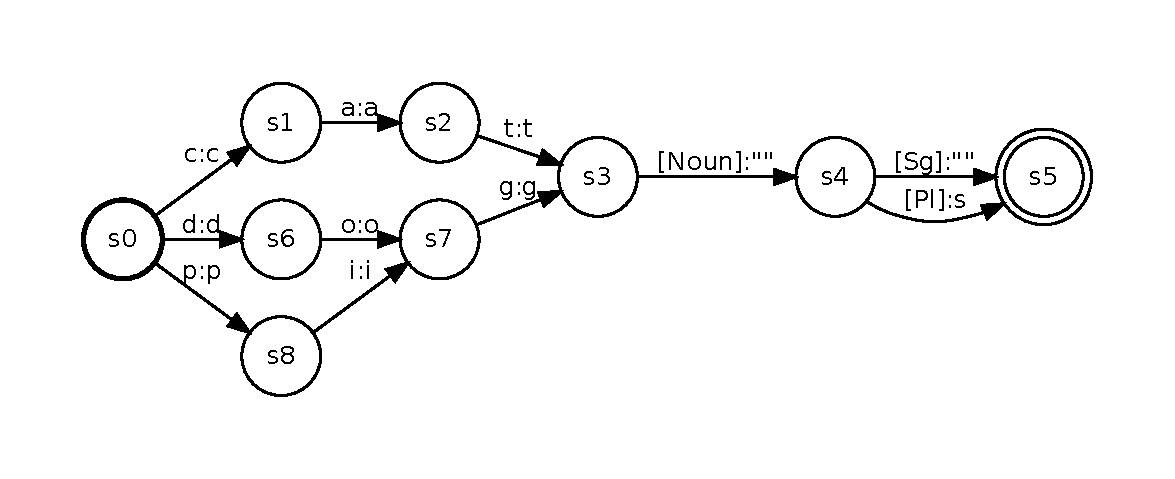
\includegraphics[width=15cm]{images/dogcatpig}
\caption{dogcatpig.pdf}
\label{fig:dogcatpig}
\end{figure}


If the transducer encodes a relation containing the pairs $<$leaf[Noun][Pl]:leaves$>$ and
$<$leave[Verb][3ps]:leaves$>$, as in Figure \ref{fig:leaves} then
applying it to ``leaves'' will first result in the
network shown in Figure \ref{fig:leavesSolution}, which will return two solutions, here leaf[Noun][Pl] and leave[Verb][3ps],
as shown in Figure \ref{fig:leavesAcc}.

\begin{figure}
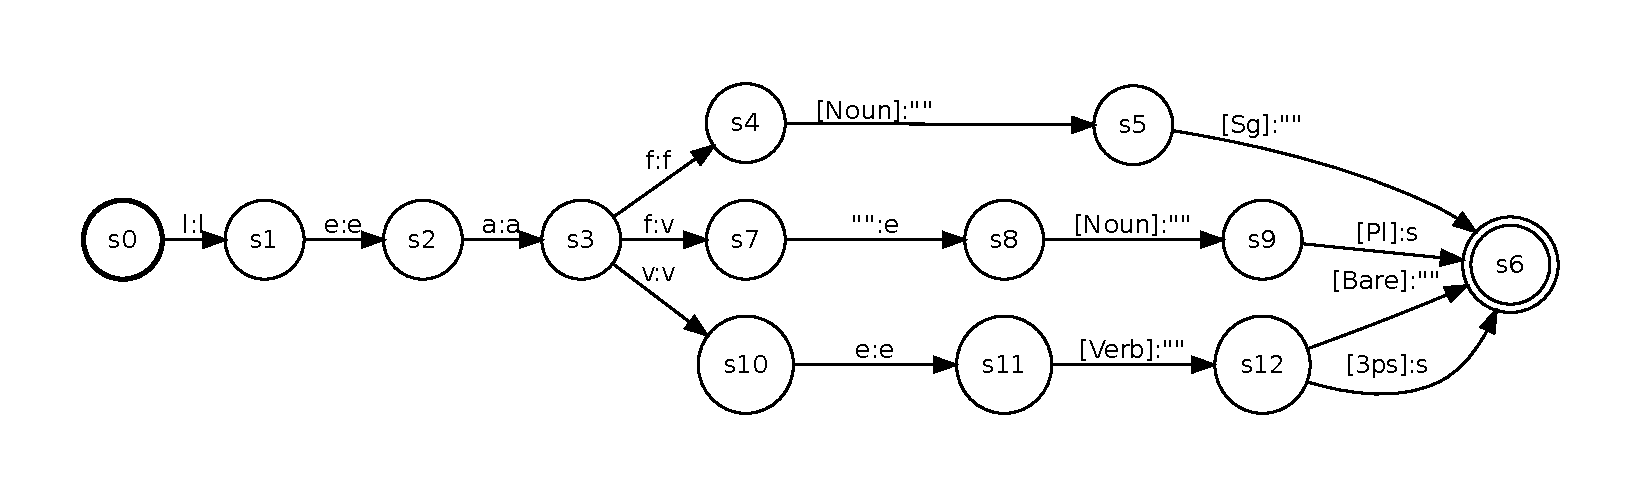
\includegraphics[width=15cm]{images/leaves}
\caption{leaves.pdf}
\label{fig:leaves}
\end{figure}

\begin{figure}
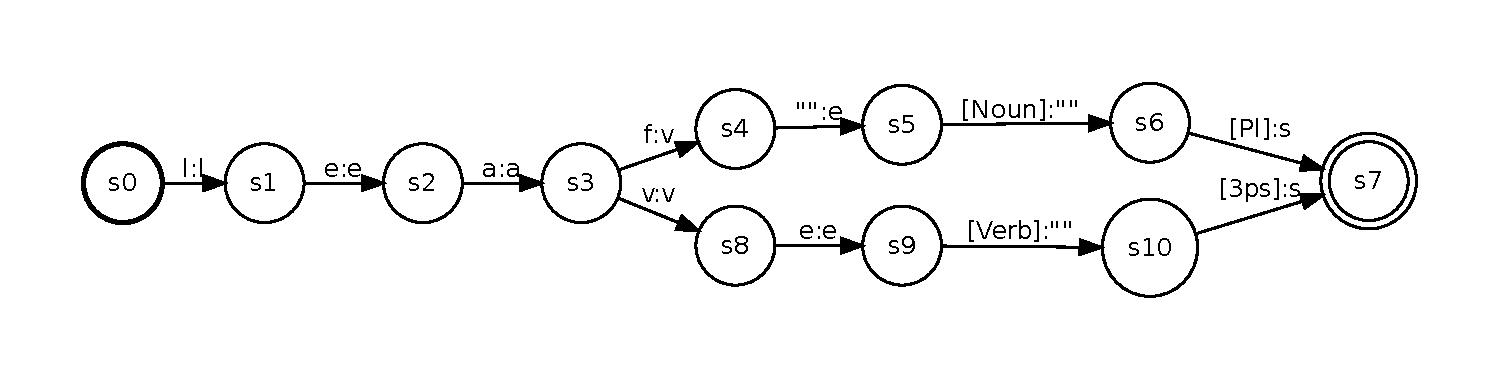
\includegraphics[width=15cm]{images/leavesSolution}
\caption{leavesSolution.pdf}
\label{fig:leavesSolution}
\end{figure}

\begin{figure}
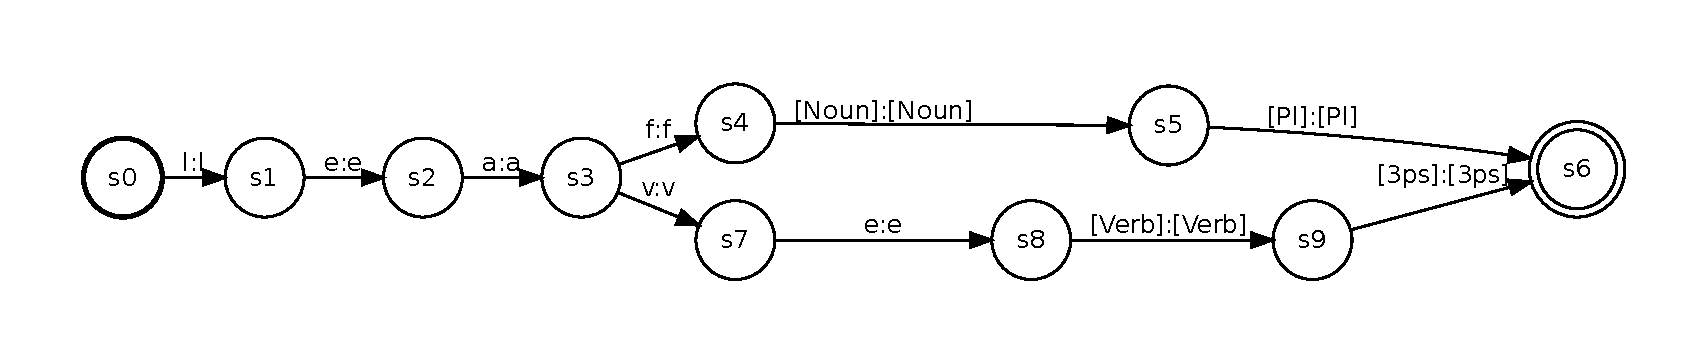
\includegraphics[width=15cm]{images/leavesAcc}
\caption{leavesAcc.pdf}
\label{fig:leavesAcc}
\end{figure}


More precisely, it is important to remember that a Transducer has two sides, and upper side and a lower
side, and when the Transducer is applied to an input string, you have to specify the direction of
application.  A transducer can be applied either ``in an upward
direction'' or ``in a downward direction'' to the input.  If the lower side encodes strings like ``cat'', and the
transducer is applied to the input ``cat'' in an upward direction, then the related upper-side string
``cat[Noun][Sg]'' will be returned.  Conversely, if the same transducer is applied in a downward
direction to the input string ``dog[Noun][Pl]'', then the related lower-side string ``dogs'' will be
returned.  Transducers are bidirectional, and so a transducer built to
encode morphological analysis
can also, using appropriate runtime code, perform morphological generation.\footnote{In the \acro{at\&t} and OpenFst traditions, one side of the transducer is
designated the Input Side and the other the Output Side, but they are still two-sided and, technically,
can be applied in either direction.}

The mathematical properties of Regular Languages and Relations, encoded as
finite-state networks, tend
to make them very computationally efficient.  While ``regular''
(finite-state) power is not sufficient to perform all
the tasks needed in natural language processing, where regular power is sufficient, developers will often go to great lengths to encode
and compute their tasks using genuinely regular networks for flexibility and computational performance.
The recognized advantages of true ``regular'' computing has led to about 50 modern projects to
implement regular/finite-state processing on
computers.\footnote{For an intimidating list, see
\url{https://kitwiki.csc.fi/twiki/bin/view/KitWiki/FsmReg}.  Most of the
projects are incomplete, poorly documented, restrictively licensed or
otherwise inappropriate for commercial use.}

\section{Regular Expressions}

\subsection{Genuinely Regular vs.~Pseudo-Regular}

Regular Expressions are a meta-language for defining Regular Languages and Regular Relations.  Here is
is vital to make a distinction between genuinely regular Regular Expression---as found in mathematical
textbooks and in a variety of programming languages including Xerox (x)fst, \acro{sfst-pl}, \acro{at\&t} Lextools and
Kleene---and pseudo regular expressions as found in general-purpose programming languages like Perl,
Python, Java, etc.; I'll call the latter Perl or Perl-like or pseudo-regular expressions.  

Perl-like regular expressions are definitely useful in many applications, but, in the classic summary, ``Perl regular
expressions aren't'', i.e.\@ they aren't truly Regular.  Perl regular
expressions do not translate into networks that can be unioned, iterated,
subtracted or composed,\footnote{In fact, Perl-like regular expressions
lack subtraction and composition operators altogether.} and Perl-like
match-and-substitute statements to not translate into
Transducers.  Perl-like regular expressions simply
do not share the attractive closure properties of regular languages/relations/networks.  A
Perl substitution expression, e.g.\@

\begin{Verbatim}[fontsize=\small]
$string ~= s/PerlRegularExpression/SubstitutionString/
\end{Verbatim}

\noindent
if it matches at all, will match in only
one way, that way often depending solidly on how the PerlRegularExpression is written, and then the matched characters
will be replaced by the SubstitutionString.  This is a kind of pattern-action semantics---match
the pattern, and trigger code that replaces the matched string with the substitution string.
This is quite different from genuine finite-state transduction.
The Perl substitution statement is an abbreviation for an
algorithmic process of matching and substitution, and that algorithm (in Perl pseudo-regular
expressions) can help itself to memory that is unavailable in a genuine regular expression.  E.g. Perl

\begin{Verbatim}[fontsize=\small]
$string ~= s/(aa|bb|cc)xyz\1)/foo/
\end{Verbatim}

\noindent
matches ``aa'' or ``bb'' or ``cc'' and then \emph{remembers} what
was matched, storing it in a special register number 1; then it continues to match ``xyz'' before finally retrieving
the pattern stored in register 1 and matching that same pattern again at the end.  Similarly, a Perl
SubstitutionString can output remembered copies of material that was matched, 
e.g.\@

\begin{Verbatim}[fontsize=\small]
$string ~= s/([a-z])([a-z])([a-z])/$3$2$1/
\end{Verbatim}

\noindent
will match a three-character string, e.g. ``abc'' and will remember `a' in
register 1, `b' in register 2 and `c' in register three; then it will
retrieve those three values and replace the matched ``abc'' with the
reversed ``cba''.  This kind of memory, however valuable it might be in
some applications, is simply unavailable in genuinely regular
systems.

\subsection{Pseudo-Regular Computing at Inxight}

In our own company history, we need to be aware that \acro{cgul} imports certain aspects of Perl-like regular
expressions that make it non-regular, and this has led to numerous serious problems, including

\begin{itemize}
\item
A loss of the notion of transduction.  \acro{cgul} patterns match, and then algorithms takes over to perform
arbitrary actions.  (\acro{cgul} patterns, like Perl regular expressions,
do not compile into transducers.  KRB: check this with Phil.)
\item
A loss of regular closure properties.  \acro{cgul} patterns cannot be combined, with reliable regular
results, in the way that genuinely regular patterns can be combined.  The
\acro{cgul} language lacks intersection altogether, and subtraction is
severely limited.
\item
A loss of typical regular performance.  Truly regular networks generally match input strings in linear
time (depending in a linear fashion on the number of arcs traversed in the
network).  Perl and other
pseudo-regular expressions (like \acro{cgul}) can easily slip into pathological cases where matching becomes
very slow.  Perl and other pseudo-regular expressions may need to be carefully rewritten to avoid or
minimize such pathological cases.  KRB:  check this with Phil.
\item
A loss of optimizability.  \acro{cgul} rule networks, with their non-regular semantics, and the
custom-written \acro{cgul} runtime code required to apply them, could not
be optimized.\footnote{Truly regular \acro{parc}
pattern matching benefits tremendously from an optimization known as Vectorization.  Non-\acro{cgul} Inxight
finite-state applications benefited from a different optimization called
fsoptimize().  But the \acro{cgul} runtime
code required that pattern networks be left full-sized.}
\end{itemize}

The Data Cleansing language from LaCrosse is another pattern-action language, very like Perl substitution statements, 
differing mainly from Perl in that it
matches and rewrites strings of \emph{tokens} rather than strings of raw \emph{characters}.  I.e. the raw string input is
first tokenized, and then it is fed to the pattern-matching and substitution actions of the Data
Cleansing language.  

\section{The Kleene Language}

\subsection{Creating Finite-state Networks}

Kleene is a programming language, a kind of development code, implemented using the JavaCC parser-generator (which generates a
Java-language parser and Abstract Syntax Tree builder), plus additional hand-written Java code that implements the
interpreter, the symbol-table environment and a \acro{gui}. 

Kleene programming is largely declarative; developers specify genuinely regular languages and regular relations using
Regular Expressions and abbreviations of Regular Expressions that include variables and function
calls.  Statements in the Kleene language, which can include genuine regular expressions,
are then parsed into Abstract Syntax Trees (\acro{ast}s), which are
interpreted to create finite-state networks, which are typically stored to file.  The interpreter builds, combines and manipulates networks
by calling algorithms in the OpenFst library.   OpenFst is written in C++, for efficiency, so the Kleene interpreter calls OpenFst functions
through the Java Native Interface (JNI).

Pre-edited Kleene scripts (created using any convenient word processor) can be processed from the command line.  The \acro{gui} offers
developers a more visual environment in which to create and visualize networks.  The output of a Kleene script, or an interactive Kleene
session, is one or more finite-state networks.  That's it.  

In the
\acro{gui}, developers can also perform limited, and not very efficient, manual testing of such networks; but once the finite-state networks
are stored to file, the job of Kleene is done.

\subsection{Limited Manual Testing inside Kleene}

Like (x)fst, and unlike \acro{sfst-pl} and Lextools, Kleene provides an interactive user interface that allows users to
build a network and then test it manually.  The user can type in individual strings to be
``analyzed'' (i.e.\@ looked up) or ``generated'', and the \acro{gui} displays the results.  This testing is done in a mathematically correct, not very efficient way that
is suitable for manual testing but would not be acceptable at runtime.  This manual testing facility should therefore not
be confused with the runtime code needed in a commercial application.

\section{Development Code vs.\@ Runtime Code}

Like the Xerox languages lexc and xfst, Kleene is a Development Tool that is used at development
time to create and finite-state networks and store them to file.  Company applications that want to integrate
finite-state processing, e.g.\@ for morphological analysis/generation, speech analysis-generation, pattern-matching, etc., don't need Kleene per se but only the networks that were produced using
Kleene.  What these applications need is Runtime Code that knows how to read in finite-state networks
and apply them to input; at runtime, Kleene is typically out of the picture.\footnote{If an application
needed to build new finite-state networks on the fly, at runtime, then it might need to integrate
Kleene, or at least OpenFst, in some way.}

Runtime Code is typically written in C++ and packaged as a library that can be linked into other
applications.  The runtime-code library would have some kind of API that would minimally contain functions to

\begin{itemize}
\item
Read in a network from file
\item
Apply that network in an upward direction to input, to perform analysis, and 
\item
Apply that network in a downward direction to input, to perform generation
\end{itemize}

\noindent
In the context of the Kleene (and Xerox) implementations, if the input is a string it must first be
`tokenized-for-application', breaking it apart into individual letters and, where appropriate, not
breaking apart strings of characters that represent multi-character symbols.  The networks will carry
with them a $\Sigma$ (sigma) that stores the alphabet of the network.

\begin{figure}
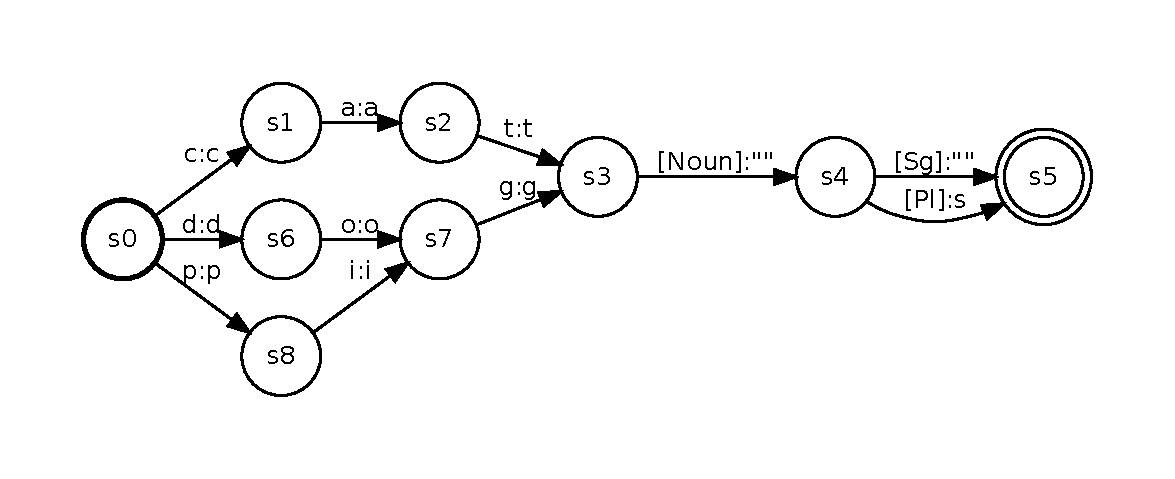
\includegraphics[width=15cm]{images/dogcatpig}
\caption{dogcatpig.pdf}
\label{fig:dogcatpig2}
\end{figure}

\begin{figure}
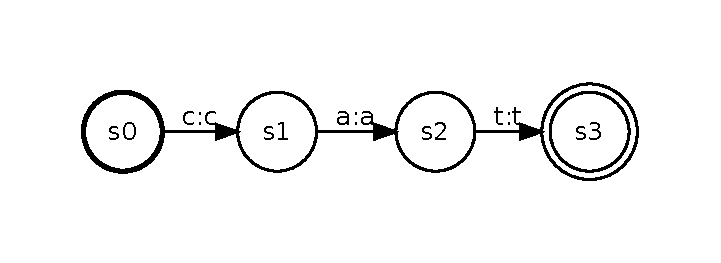
\includegraphics[width=15cm]{images/cat}
\caption{cat.pdf:  The input string ``cat'' converted into a one-string acceptor network.}
\label{fig:cat}
\end{figure}

\begin{figure}
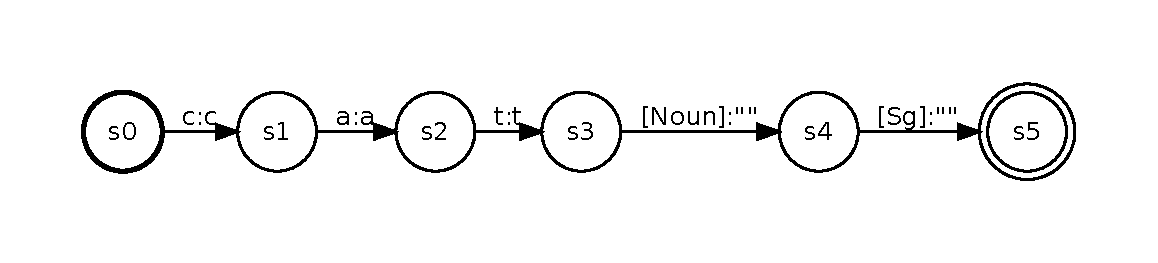
\includegraphics[width=15cm]{images/catNounSg}
\caption{catNounSg.pdf: The result of composing \$dogcatpig with
\$InputNet on the lower side.}
\label{fig:catNounSg}
\end{figure}

\begin{figure}
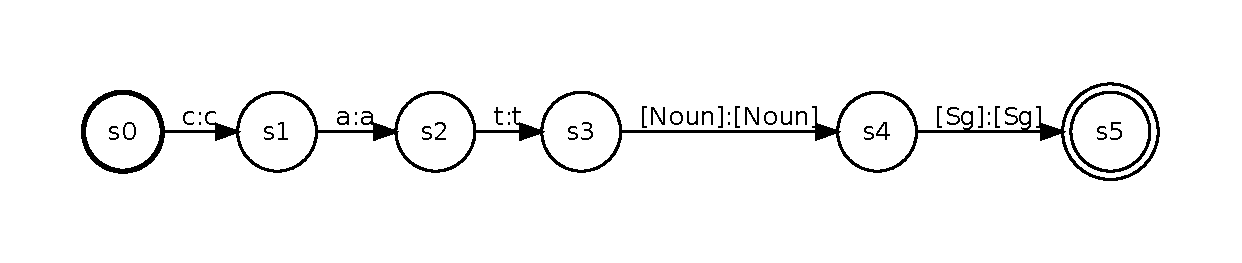
\includegraphics[width=15cm]{images/catNounSgAcc}
\caption{catNounSgAcc.pdf:  The upper-side language of the result.  In the OpenFst implementation,
all labels are two-level, and an acceptor is a special case of a transducer wherein all the
input:output labels are identity mappings.}
\label{fig:catNounSgAcc}
\end{figure}



\section{Applying Networks to Input}

\subsection{Application using Finite-State Algorithms}

When we talk about applying networks to input, we need to distinguish between 
mathematically-correct application using finite-state algorithms, and the much more efficient
implementation of application in Runtime Code.  We'll first look at mathematically-correct
application using finite-state algorithms.


Assume that we start with the network created by the following expression.  The following statements
can be typed into the Kleene interface.

\begin{Verbatim}[fontsize=\small]
$network = (dog|cat|pig) '[Noun]':"" ( '[Sg]':"" | '[Pl]':s ) ;
draw $network ;
\end{Verbatim}

\noindent
and the resulting network is shown in Figure \ref{fig:dogcatpig2}.
Intuitively, if you use this network to analyze the string ``rat'', then
the output should be the string ``rat[Noun][Sg]'',
and if you use this same network to generate ``elephant[Noun][Pl]'', then the output should be
``elephants''.  This can be tried in the Kleene \acro{gui} using the `test' command

\begin{Verbatim}[fontsize=\small]
test $network ;
\end{Verbatim}

\noindent
which brings up a special testing window.

When you enter ``cat'' in the lower-side entry field of the test window, to look up ``cat'', here is what is happening
underneath:

\begin{enumerate}
\item
The input string ``cat'' is read and split up into an array of int, each int representing the Unicode code
point value of a symbol.  In this case, the symbols are all standard Unicode characters, and the
ints are (in hex) 0x63, 0x61 and 0x74.
\item
This array of int is passed to a native (C++) function that literally builds a one-string finite-state network with arcs
labeled (starting from the start state) 0x63, 0x61 and 0x74.  (The labels on OpenFst arcs are integers.)
Lets call this, using the Kleene \$-sigil notation, the \$InputNetwork, which (with integer
labels
shown as characters) is shown in Figure \ref{fig:cat}.
\item
The \$InputNetwork is then composed on the lower-side of the \$network, creating the new network
shown in Figure \ref{fig:catNounSg}.  Then the upper-side (or ``upper projection'') language is
extracted, as in the following pseudo-code: \$\&upperside(\$network \_o\_ \$InputNetwork).  The
final network result is shown in Figure \ref{fig:catNounSgAcc}.
\item
The resulting network, in this case, encodes the single string ``rat[Noun][Sg]''.  A native (C++)
function (listAllStrings()) is then called to traverse or ``walk'' this network, printing all the strings in the
History Windows.
\end{enumerate}

\noindent
For generation, the process is exactly the same except that in step 3 the InputNetwork is composed on the \emph{top}
side of \$network, and the lower-side of the result is extracted, i.e.\@ \$\&lowerside(\$InputNetwork
\_o\_ \$network).
In the Kleene \acro{gui}, try entering ``cat[Noun][Pl]'' in the upper-side input field.  

The mathematically-correct implementation of application, implemented in the Kleene \acro{gui}
\texttt{test} command, therefore reduces to 
composition and
extraction of the opposite-side projection.  The InputNetwork in these cases was a single-string
network, produced from a single input string, but in general the input network could be any Acceptor,
or even another Transducer.  The composition could be empty, and if not empty, the output projection
would have one or more (even an infinite number of) strings.

This is the clean, general and mathematically correct way to do application, and this is literally what is
happening when you enter words in the `test' window in the Kleene \acro{gui}.  This same
mathematically correct approach is used to implement the
\texttt{testWordlistFile} command, which reads input strings from a designated file (one string per line), and outputs
the results to an \acro{xml} file.

Note, again, that the input network composed with the base network during application is \emph{not} limited to
representing a language of only one string.  In fact, the input could be any Acceptor encoding a regular language, or it
could even be a Transducer representing a regular relation.  If the input
is encoded as a
Language or Relation, then it can represent ambiguous readings of the input.

The only problem with this approach is that building the \$InputNetwork, performing a composition,
extracting one projection, and walking it to produce the output strings, is all rather expensive
computationally.  In the \acro{gui}, where the user is typing in one input string at a time, or
where the input is in a relatively small wordlist file, it's good enough;
but in a commercial application the performance would be unacceptably slow.

\subsection{Runtime Code for Better Performance}

Where in mathematically correct application (and the manual testing facility in the Kleene \acro{gui}) 

\begin{enumerate}
\item
The input is encoded as a finite-state network
\item
The input is composed with the base network, creating a new result Transducer
\item
One projection of the result network is extracted, creating a result Acceptor, and
\item
The result Acceptor is then ``walked'' to print out the strings
\end{enumerate}

\noindent
in practical runtime code these operations are \emph{simulated} in C++ code achieve far greater efficiency.

In runtime code, the input (which might be a simple string, or a linked list of some sort, or
whatever) might be traversed directly in its native form---i.e.\@ there is no necessary
requirement to convert it into a finite-state network.  And the runtime code knows how to
traverse the network itself, at the state and arc level, matching input symbols against arc
labels, ``remembering'' the output symbols, and backtracking wherever appropriate to find all
possible solutions.

Complications include 

\begin{enumerate}
\item
Accumulating weights along paths (using the ``extension''
operation\footnote{The extension operation is called Times() in OpenFst.} of the applicable
semiring.
\item
Handling epsilons.
\item
Handling networks that have been compressed or optimized-for-speed (see below).
\end{enumerate}

\section{Kinds of Runtime Code}

\subsection{Full-string Matching}

Runtime code that performs full-string matching, as needed in morphological analysis and generation, has the following high-level behavior, first looking
at analysis:

\begin{enumerate}
\item
The input string, e.g.\@ ``rat'',  is first split up and converted into an array of int, each int representing the Unicode code
point value of a character.
\item
The runtime code traverses the network directly, at low levels, matching the ints directly against the labels on
the lower side of arcs (in the Xerox visualization), or perhaps against the input-side labels (in the OpenFst
visualization).
\item
The labels on the upper (Xerox) or output (OpenFst) side of matched arcs are collected/concatenated as the matching progresses along a path, and the
weights along the path are accumulated (using the extension or Times() operation of the
applicable semiring).
\item
When the matching process successfully reaches a final state, the result string and its weight are
output.
\item
The runtime code handles epsilon arcs and other decision points, backtracking as necessary to output
all the result strings (and their weight).
\end{enumerate}

\noindent To perform generation, the process is the same, except that the integers are matched against the upper-side
labels (in the Xerox visualization), or the output-side labels (in the OpenFst visualization), and the labels on the
lower side of the matched path are collected/concatenated to form the result string(s).

{\bfseries In short, Runtime Code for full-string matching \emph{simulates} the composition and projection-extraction of the
mathematically-correct approach, with much improved performance.}

While we usually think of morphological analysis and generation in terms of ``applying a network to an input string'', we
have already seen that there is no mathematical reason to limit the input to a single string.  The input, in general
application, could be a Regular Language or a Transducer.

\subsection{Multiple Matching of Patterns within the Input}

In contrast to the full-string matching just described, there are applications where the matching strategy requires
Partial Matching: trying to match a pattern, or a set of patterns, multiple times within the same input.  The output may
show multiple matches, and parts of the input may not be matched at all.  An obvious simple example of such Partial
Matching would be looking for all occurrences of a name, e.g. \emph{Barack Obama} within a file.

A good example of one pattern-matching strategy is documented in the paper \emph{Pattern
Matching and Other New Functionality in \acro{parc} fst 2.9.5+}.\footnote{Copy available on request.}
In a nutshell, the \acro{parc} approach is to define relatively simple patterns, which can be
trivially unioned together into one comprehensive pattern network.  The
input, at \acro{parc}, is
a simple string of characters, not tokenized or marked up in any way, 
and the runtime code starts by placing a
match-pointer at the beginning of the input stream and trying to match (simultaneously) all the
patterns starting from that match-point.

Of course, multiple patterns might match, starting at the match-pointer, and the \acro{parc}
Matching Strategy is to prefer the longest match.  This strategy is built into the runtime code,
not into the individual rules.\footnote{xfst has ``longest match'' rules that prefer longest
matches in purely finite-state terms, but they get very large very fast.  Lauri Karttunen moved
the support of the longest-match preference from the rules/patterns themselves to the more
efficient and compact runtime code.}  There are some user options, but in broad strokes

\begin{enumerate}
\item
If there are matches, the longest match is retained, shorter matches are discarded, and the
match pointer is moved after the end of the matched text.
\item
If there are no matches, the match-pointer is moved ahead, usually by one orthographical word.
\end{enumerate}

\section{Runtime Code must be Intimately Tied to ``Final'' Compressions and Speed Optimizations}

\subsection{Standard Networks vs.~``Final'' Modified Networks}

\subsubsection{Built-in Standard Optimizations}

The networks produced by Kleene (via OpenFst) could be called Standard Format or full-sized networks.
They may be reduced somewhat in size via the following three built-in OpenFst optimizations 

\begin{itemize}
\item
Determinize
\item
Minimize
\item
RmEpsilon (remove epsilon:epsilon arcs)
\end{itemize}

\noindent
but these three operations still leave a Standard Format network that can be used in further operations
(such as union, concatenate, compose, etc.).  These same three
built-in optimizations are also used the Xerox/\acro{parc}
implementation.

\subsubsection{More Aggressive, Non-standard, ``Final''
Optimizations}

In addition to these standard optimizations, some implementations of
finite-state networks may also invent
more aggressive ``final'' optimizations to reduce the size or improve the runtime performance of
networks.  (In general, reducing the size slows performance, and optimization for speed increases the size.)
Typically, after a network undergoes one of these ``final'' operations, it is no longer in
Standard Format and can no longer be used in operations such as concatenation, union and composition;
it may be possible for the algorithms to detect the final optimizations and undo them (returning a
network to Standard Format) before performing further finite-state operations on the network.

These aggressive final optimizations are non-standard,
idiosyncratic, and highly dependent on the needs and skills of a
particular development group.
For example, the \acro{parc} (Xerox) implementation includes an
important optimization-for-speed called Vectorization that identifies states with
a large number of exit arcs (by default, 10 or more) and replaces those arc sets with an arc vector.
Iterating through a large set of exit arcs, looking for a match or matches with the current symbol is
rather inefficient; in contrast, the arc vector allows quick one-step lookup to find any matches.  \acro{parc} also
includes a ``Karttunen Compaction'' algorithm that physically reduces the size of a network, which is
often vital in commercial applications with memory limitations.  Optimization for speed usually
increases the size of a network, and optimization for size usually slows performance.\footnote{Xerox
also offered a ``Kaplan Compression'' algorithm, which was re-implemented
at Inxight as fsoptimize().  This
Kaplan Compression involves an extremely radical transformation of a network that requires completely
rewritten (and very tricky) runtime code; and a Kaplan Compressed network cannot be un-compressed.  Few
people apart from Ron Kaplan have ever understood Kaplan Compression, and
it's possible that fsoptimize() is
still buggy; certainly Inxight developers found it very difficult to
predict and control what fsoptimize()
would do.  Even Lauri Karttunen never wanted to deal with Kaplan Compression, and at \acro{parc} and
its spin-off Powerset, Kaplan Compression is not used at all.}

Xerox/\acro{parc} Vectorization (for speed) and Karttunen Compaction (for size) can both be undone, leaving a
standard-format Xerox network that can then be used in further finite-state
operations. fsoptimize(), implementing the
aggressive Kaplan Compression algorithm, results in such a radically restructured network (a kind of depth-first
linearization, stored as a plain text file) that it cannot even be undone.  Runtime code has to be modified to handle vectorization and Karttunen
Compaction; and runtime code to handle a Kaplan-compressed network
is especially nasty to write.\footnote{Runtime code to handle
fsoptimize()-compressed networks was written at Inxight, probably by Mike
Wilkens, now long gone.}

Here's the important point:  Any ``final'' optimization (for speed or for size) modifies the structure
of a network, perhaps radically, and must be closely coordinated with the Runtime Code that will apply
that network to input.  In practice, a ``final'' optimization and the Runtime Code that knows how to
handle the modified networks must be developed in parallel, ideally by the same person.

\subsection{Overlaps between Development Code and Runtime Code}

The cleanest design would make a strict separation between development code (Kleene) that creates
Standard Format networks
and stores them to file, vs.\@ post-processing that includes any ``final'' optimizations and their
coordinated Runtime Code.  

If any final compression/optimization is performed, these would be done outside of
Kleene, and each compression/optimization operation would be tightly coordinated with the
Runtime Code needed to understand the modified network structures.  E.g.\~ if (for Kleene/OpenFst) we design an
aggressive compression algorithm (similar to Fsopt() (``Kaplan Compression'') or ``Karttunen
Compaction'' or Vectorization in the Xerox/parc implementation) then we will need to write parallel runtime code
that knows how to read and apply the modified networks.

Once an aggressive ``final'' optimization is devised, with suitable coordinated Runtime Code, then it would be
theoretically possible to migrate these final optimizations back into Kleene itself, so that such optimized networks could be
created and saved to file by Kleene.  E.g.\@ if we invent a PhilCompression
or PaolaSpeedOptimization algorithm, then these algorithms might
eventually be incorporated into Kleene so that Kleene
developers could invoke the algorithms and save networks in these finally-optimized formats.  The coordinated Runtime Code could
also, theoretically, be migrated into Kleene to allow such finally-optimized networks to be tested in the Kleene GUI.

However, I believe that such migrations should be approached very cautiously, and probably avoided.
Keeping the clean division between Kleene and Standard Format networks vs.\@ Runtime Code and Final
Optimizations has the following advantages: 

\begin{itemize}

\item
Kleene would remain more stable while allowing unlimited experimentation in the final
optimizations and Runtime Code.
\item
The separation promotes a healthy modularity, 
allowing different people and different teams to work on Kleene proper vs.\@
compression/optimization and Runtime Code.
\item
The modularity would also extend to the documentation.
\item
Kleene proper (destined to be an open-source project released under the Apache license) could remain a
stand-alone, distributable programming language without needing to expose proprietary final
compressions/optimizations and the Runtime Code.
\end{itemize}

\section{Afterthoughts}

\subsection{Tokenization for Application}

The tokenization-for-application, which reduces an input string to an array of int (Unicode code point
values) is not as simple as described above.  In particular, when the network contains multi-character
symbols like [Noun], [Sg] and [Pl], then the tokenization-for-application must keep them together and
assign them a single code point value.  If the string input is rat[Noun][Pl], consisting of 13 characters, and if [Noun]
and [Pl] are multi-character symbols in the network being applied, then the tokenization-for-application should recognize
only five symbols

\begin{itemize}
\item
r
\item
a
\item
t
\item
\verb![Noun]!
\item
\verb![Pl]!
\end{itemize}

\noindent
and assign a single code-point value to each symbol.
In the Kleene system, symbols like \emph{r}, \emph{a} and \emph{t} are
automatically assigned their standard Unicode code point values, and multicharacter symbols are
assigned code point values from a Unicode Private Use Area (\acro{pua}). 

In the current Kleene `test' and `testWordlistFile' facilities, the tokenization-for-application is
performed using Transliterator objects from the \acro{icu4j}
library.  This `tokenization-for-lookup' code, already running in
the Kleene \acro{gui}, could be extracted for use in runtime
code.\footnote{The Kleene \acro{gui} uses Transliterator objects
from \acro{icu4j}, which is Java code, but \acro{icu} also exists
for C++.}

\subsection{A More Aggressive View of the \acro{api}}

A more aggressive view of the \acro{api} would have it include
operations beyond the application of a single network to input.  In
particular, it might be useful to have runtime code capable of
reading multiple networks, and keeping them separate, but applying
them to input \emph{as if they were composed together}.  In other
words, it is often useful to have runtime code that can
\emph{simulate} the composition of networks at runtime.

The composition of two networks can, in the worst case, result in a
network that has a number of states equal to the product of the
states in the two original networks.  In short, composition of two
or more networks can all too easily result in an explosion in size.

OpenFst allows delayed or ``lazy'' operations that take two networks
and constructs the result (e.g.\@ the composition) incrementally,
only as much as needed to handle the actual input.

Xerox also had runtime code that could simulate composition at
runtime.

\subsection{The Most Aggressive View of the \acro{api}}

The most aggressive view of the \acro{api} would allow full creation
and manipulation of networks from within an existing programming
language like Java, Python or Ruby.  In the last year or two, this
has been done at \acro{parc} and their spin-off Powerset.  

I'm not very sympathetic to this approach, but apparently it was
popular at Powerset, where everyone programs in Ruby, and the
developers wanted to create and manipulate finite-state networks
without getting out of Ruby to program in lexc and/or xfst.

\section{Converting Networks to Stand-alone Executable Code}

A radical approach to applying networks involves taking a finite-state network
and converting it directly into stand-alone 
executable code, e.g.\@ a Java or C++ class.  For
example, in Java code, you would create an instance of the class, 

\begin{Verbatim}[fontsize=\small]
    MyNetwork myNetwork = new MyNetwork() ;
\end{Verbatim}

\noindent
and that class would provide a convenient method like

\begin{Verbatim}[fontsize=\small]
    ArrayList<String> analyze(String input)
\end{Verbatim}

\noindent
that takes an input String, tokenizes it for analysis, analyzes it, and
returns
a list of String results.  The user code would then simply make calls like
the following

\begin{Verbatim}[fontsize=\small]
    ArrayList<String> resultList = mynetwork.analyze("dog") ;
\end{Verbatim}


A new class would have to be created for each
network, and separate classes would need to be created for analysis vs.\@
generation; but for many users needing full-string matching this approach
would be the easiest for integrating finite-state processing into larger
systems.

In practice, the user would create a network \verb!$myNetwork! in Kleene, test it, and then
invoke a single Kleene command such as

\begin{Verbatim}[fontsize=\small]
createJavaAnalysisClass $myNetwork, "MyNetwork.java" ;
\end{Verbatim}

\noindent
or
\begin{Verbatim}[fontsize=\small]
createJavaGenerationClass $myNetwork, "MyNetwork.java" ;
\end{Verbatim}

\noindent
and the Java class would be ready to use.

The generated class would need to incorporate tokenization-for-application,
and it would have one method representing each state in the original
network, with a \texttt{switch} statement in each method.  

I successfully converted Xerox-style networks into executable Java
code, implementing full-string matching, in 2007, and the same work could be done for Kleene/OpenFst networks.


\end{document}
